\documentclass[a4paper,
fontsize=11pt,
%headings=small,
oneside,
numbers=noperiodatend,
parskip=half-,
bibliography=totoc,
final
]{scrartcl}

\usepackage[babel]{csquotes}
\usepackage{synttree}
\usepackage{graphicx}
\setkeys{Gin}{width=.8\textwidth} %default pics size

\graphicspath{{./plots/}}
\usepackage[ngerman]{babel}
\usepackage[T1]{fontenc}
%\usepackage{amsmath}
\usepackage[utf8x]{inputenc}
\usepackage [hyphens]{url}
\usepackage[hyphenbreaks]{breakurl}
\usepackage{booktabs} 
\usepackage[left=2.4cm,right=2.4cm,top=2.3cm,bottom=2cm,includeheadfoot]{geometry}
\usepackage{eurosym}
\usepackage{multirow}
\usepackage[ngerman]{varioref}
\setcapindent{1em}
\renewcommand{\labelitemi}{--}
\usepackage{paralist}
\usepackage{pdfpages}
\usepackage{lscape}
\usepackage{float}
\usepackage{acronym}
\usepackage{eurosym}
\usepackage{longtable,lscape}
\usepackage{mathpazo}
\usepackage[normalem]{ulem} %emphasize weiterhin kursiv
\usepackage[flushmargin,ragged]{footmisc} % left align footnote
\usepackage{ccicons} 
\setcapindent{0pt} % no indentation in captions

%%%% fancy LIBREAS URL color 
\usepackage{xcolor}
\definecolor{libreas}{RGB}{112,0,0}

\usepackage{listings}

\urlstyle{same}  % don't use monospace font for urls

\usepackage[fleqn]{amsmath}

%adjust fontsize for part

\usepackage{sectsty}
\partfont{\large}

%Das BibTeX-Zeichen mit \BibTeX setzen:
\def\symbol#1{\char #1\relax}
\def\bsl{{\tt\symbol{'134}}}
\def\BibTeX{{\rm B\kern-.05em{\sc i\kern-.025em b}\kern-.08em
    T\kern-.1667em\lower.7ex\hbox{E}\kern-.125emX}}

\usepackage{fancyhdr}
\fancyhf{}
\pagestyle{fancyplain}
\fancyhead[R]{\thepage}

% make sure bookmarks are created eventough sections are not numbered!
% uncommend if sections are numbered (bookmarks created by default)
\makeatletter
\renewcommand\@seccntformat[1]{}
\makeatother

% typo setup
\clubpenalty = 10000
\widowpenalty = 10000
\displaywidowpenalty = 10000

\usepackage{hyperxmp}
\usepackage[colorlinks, linkcolor=black,citecolor=black, urlcolor=libreas,
breaklinks= true,bookmarks=true,bookmarksopen=true]{hyperref}
\usepackage{breakurl}


%meta
%meta

\fancyhead[L]{F. Corradini\\ %author
LIBREAS. Library Ideas, 38 (2020). % journal, issue, volume.
\href{http://nbn-resolving.de/}
{}} % urn 
% recommended use
%\href{http://nbn-resolving.de/}{\color{black}{urn:nbn:de...}}
\fancyhead[R]{\thepage} %page number
\fancyfoot[L] {\ccLogo \ccAttribution\ \href{https://creativecommons.org/licenses/by/4.0/}{\color{black}Creative Commons BY 4.0}}  %licence
\fancyfoot[R] {ISSN: 1860-7950}

\title{\LARGE{Einfluss der Agenda 2030 auf die deutschsprachige Bibliothekswelt}}% title
\author{Franziska Corradini} % author

\setcounter{page}{1}

\hypersetup{%
      pdftitle={Einfluss der Agenda 2030 auf die deutschsprachige Bibliothekswelt},
      pdfauthor={Franziska Corradini},
      pdfcopyright={CC BY 4.0 International},
      pdfsubject={LIBREAS. Library Ideas, 38 (2020).},
      pdfkeywords={Bibliothek, IFLA, Klimaschutzbewegung, Schweiz, Deutschland, Ziele für nachhaltige Entwicklung},
      pdflicenseurl={https://creativecommons.org/licenses/by/4.0/},
      pdfcontacturl={http://libreas.eu},
      baseurl={http://libreas.eu},
      pdflang={de},
      pdfmetalang={de}
     }



\date{}
\begin{document}

\maketitle
\thispagestyle{fancyplain} 

%abstracts

%body
Genau wie Libraries4Future sieht auch die International Federation of
Library Associations and Institutions (IFLA) Bibliotheken in einer
Schlüsselrolle für eine klimafreundliche und friedliche Welt.
Nachhaltigkeit gehört schon lange zum Themenrepertoire der IFLA. Dadurch
konnte sie bei der Entstehung der Agenda 2030 soweit Einfluss nehmen,
dass in dieser der Zugang zu Information, Kommunikations- und
Informationstechnologien als Zielelemente verankert sind. (IFLA, 2015,
S. 5)

Die Agenda 2030 ist ein Katalog aus 17 Zielen für Nachhaltige
Entwicklung, die bis 2030 erreicht werden sollen.\footnote{\url{https://sdgs.un.org/goals}.}
Dadurch sollen sowohl Menschen als auch der Planet zu Frieden und
Wohlstand kommen. Alle Mitgliedstaaten der Vereinten Nationen haben die
Agenda 2030 im Jahr 2015 unterzeichnet und sind nun daran, die Ziele
umzusetzen.

Wie hat sich die Veröffentlichung der 17 Ziele für Nachhaltige
Entwicklung (alias Agenda 2030) auf die deutschsprachige Bibliothekswelt
ausgewirkt? Diese Frage habe ich im Rahmen meiner
informationswissenschaftlichen Bachelorarbeit an der Fachhochschule
Graubünden (FHGR) untersucht. Als Methodik wählte ich die Fallstudie und
setzte dies mittels einer Literaturrecherche um. Die Ergebnisse sind in
einer öffentlichen Zotero-Bibliothek\footnote{\url{https://www.zotero.org/groups/2450268/einfluss_der_sdgs_auf_bibliotheken}.}
abgelegt.

\begin{figure}
\centering
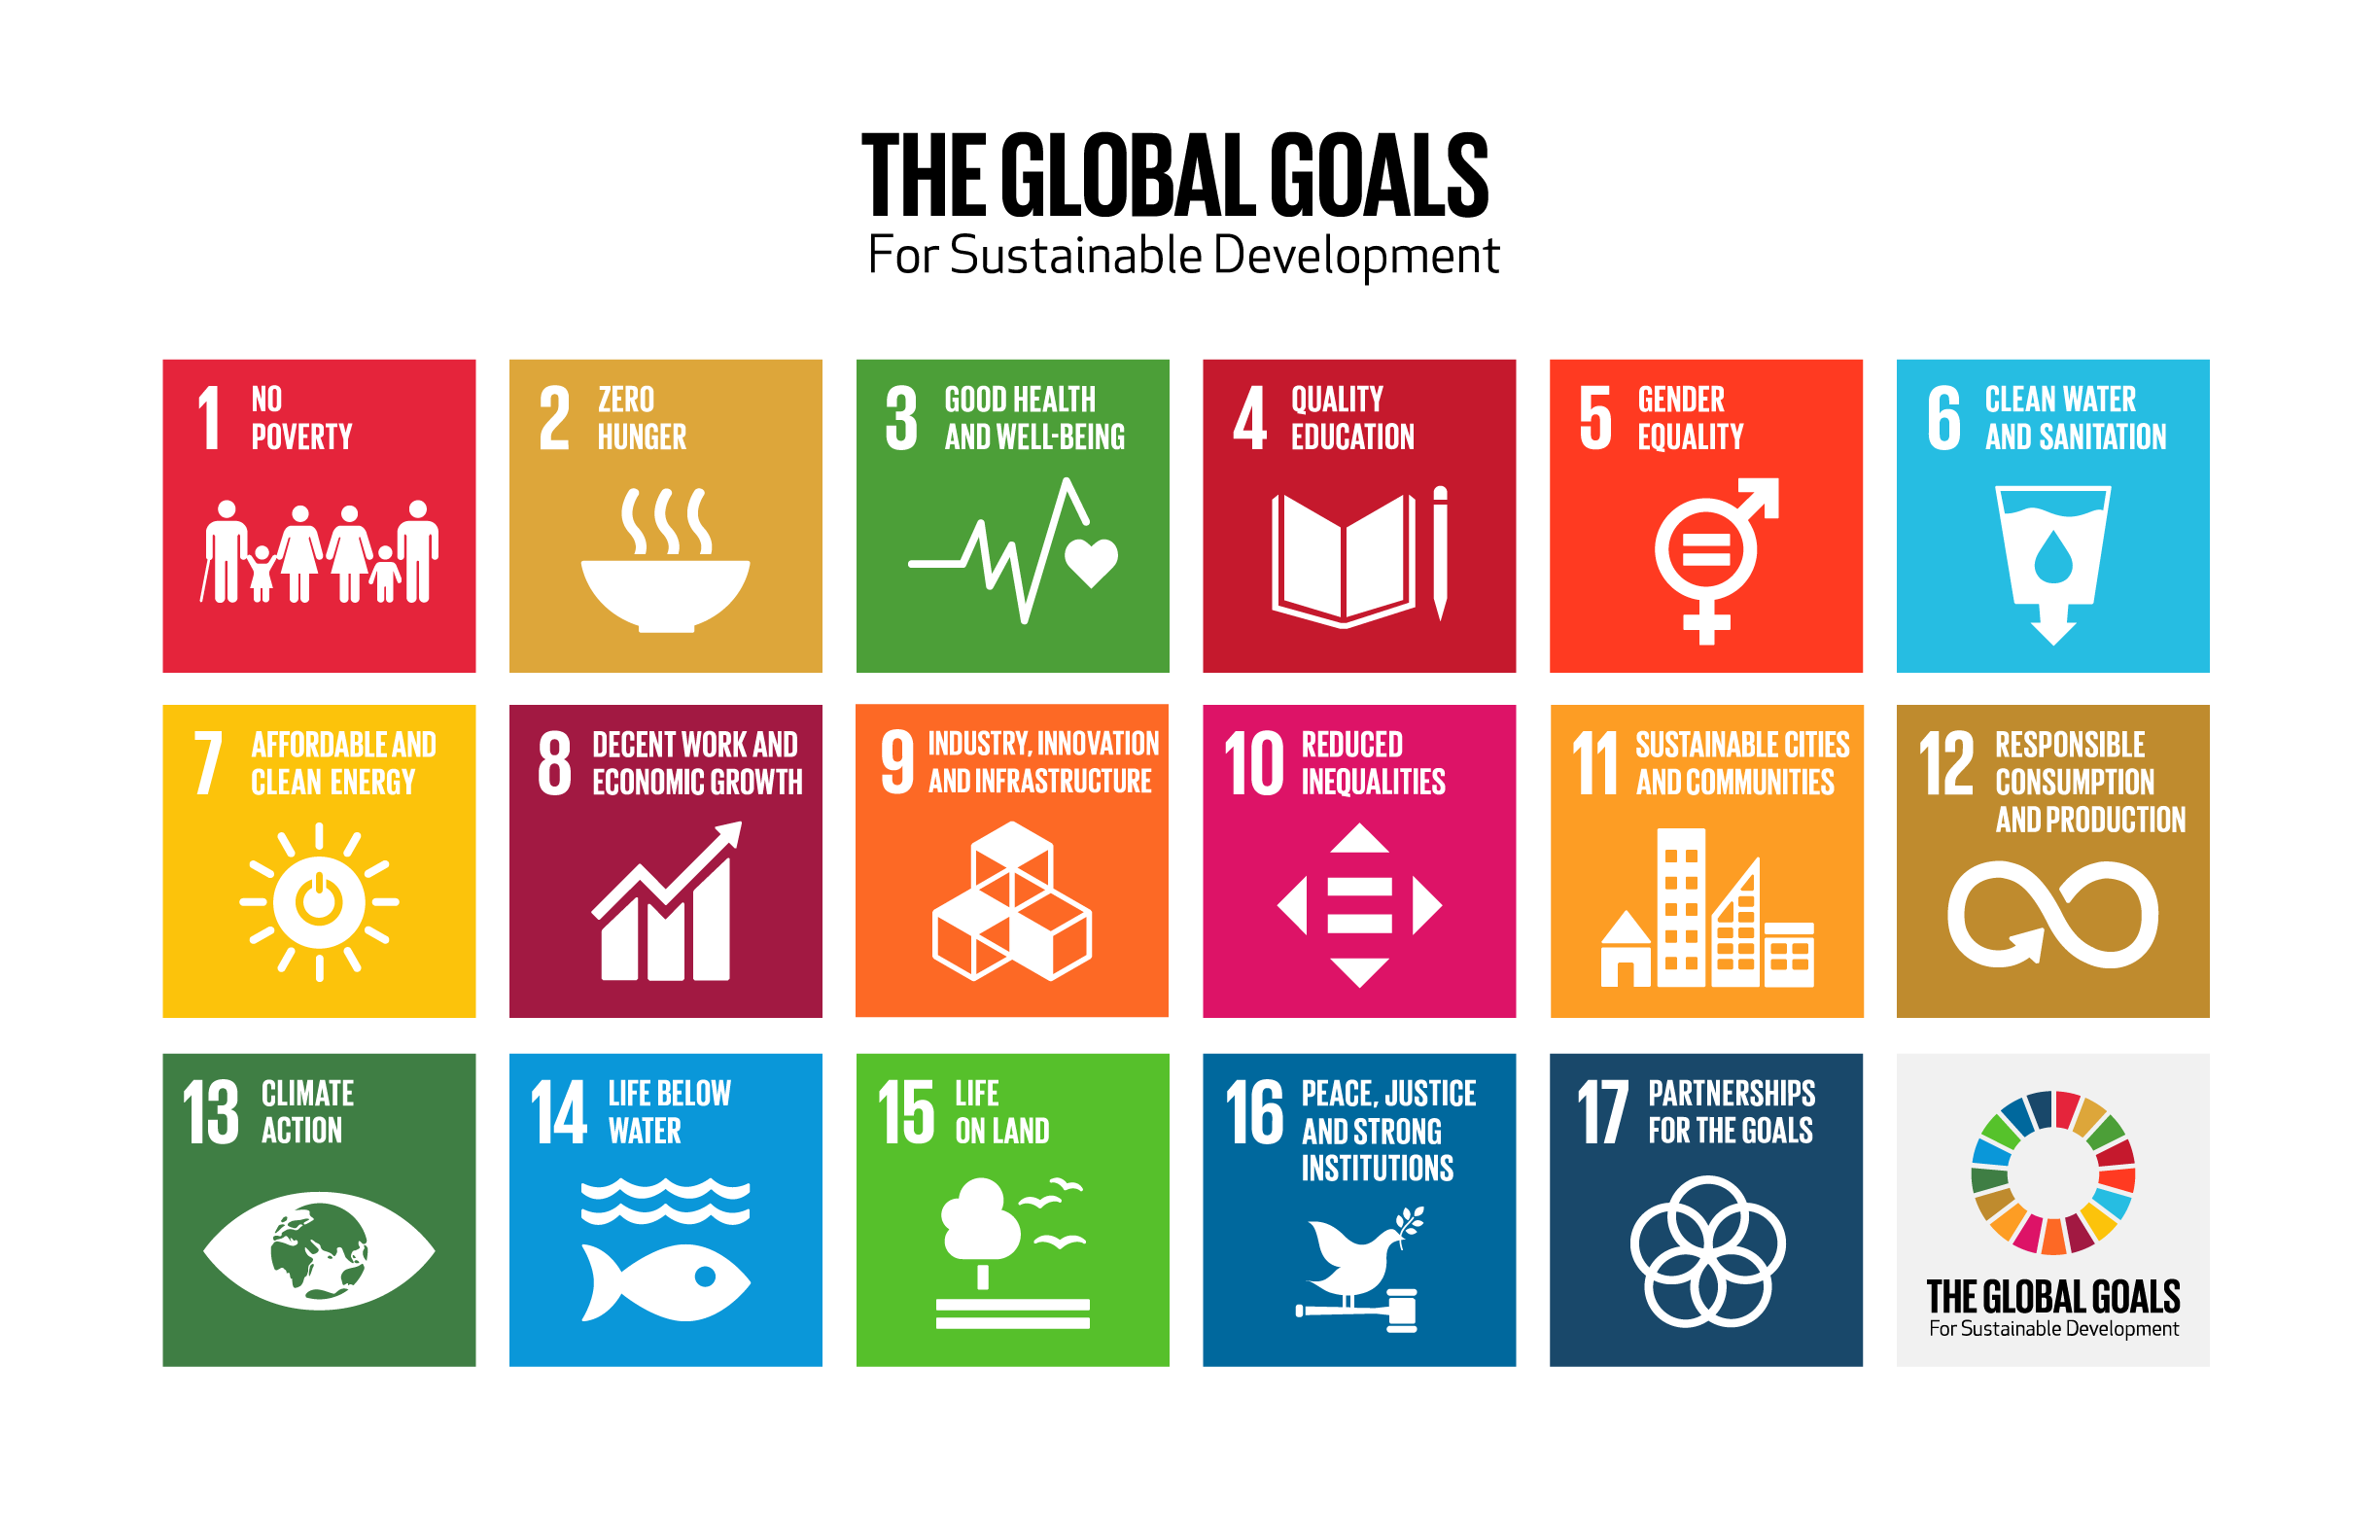
\includegraphics{img/sgd_17.png}
\caption{Die 17 SDGs (United Nations, o.J.)}
\end{figure}

\hypertarget{die-ifla-pruxe4gt-den-einfluss-der-agenda-2030-auf-bibliotheken}{%
\section{Die IFLA prägt den Einfluss der Agenda 2030 auf
Bibliotheken}\label{die-ifla-pruxe4gt-den-einfluss-der-agenda-2030-auf-bibliotheken}}

Die IFLA verfolgte den Entstehungsprozess der Agenda 2030 genau. Sie
setzte sich dafür ein, dass der Zugang zu Information in den Zielen für
Nachhaltige Entwicklung vorkommt. Als diese 2015 veröffentlicht wurden,
publizierte die IFLA zeitnah einen Werkzeugkasten, wie die Bibliotheken
zur Erfüllung der Ziele für Nachhaltige Entwicklung beitragen können.
Das prägte die Entwicklung im Bibliotheksraum massgebend. Das Dokument
wurde von den verschiedenen Bibliotheksverbänden aufgenommen,
gegebenenfalls etwas adaptiert und so gut als möglich umgesetzt.

Die IFLA verfolgte mit dem Werkzeugkasten ein Ziel: Bibliotheken sollen
in den nationalen Strategien zur Erreichung der Agenda 2030 als
Partnerinnen genannt werden. Aus Sicht der IFLA waren darum zunächst die
Bibliotheksverbände gefragt, allenfalls ergänzt durch
Bibliotheksmitarbeitende, welche auf nationaler Ebene tätig sind. Diese
sollten durch Öffentlichkeits- und Interessensarbeit die politischen
Entscheidungsträger überzeugen, dass Bibliotheken wichtige
Kooperationspartnerinnen für die Umsetzung der Agenda 2030 sind.

Um das zu erreichen, rief die IFLA das International Advocacy Programm
(IAP) ins Leben. Sie definierte folgende Ziele:

\begin{quote}
"Raise the level of awareness on the SDGs of library workers at
community, national and regional levels, and to promote the important
role libraries can play in development by contributing to the UN 2030
Agenda and the SDGs;

Increase the participation of library associations and public library
representatives in advocacy work at national and regional levels to
secure sustainable public access to information through library services
and programmes." (IFLA, 2020)
\end{quote}

Im IFLA Werkzeugkasten spielten die einzelnen Bibliotheksmitarbeitenden
eher eine untergeordnete Rolle. Erst auf der letzten Seite wurden sie in
einem Satz erwähnt, erhielten damit aber den umfassenden Auftrag alle
Bibliotheksnutzerinnen und -nutzer über die Agenda 2030 und die Ziele
für Nachhaltige Entwicklung aufzuklären. (IFLA, 2015, S. 15)

Trotz dieses Auftrags gibt es kaum Materialien, welche Bibliotheken in
der konkreten Vermittlung unterstützen oder sie dazu animieren. Für die
einzelnen Bibliotheken hat die IFLA die Plattform Library Map of the
World erstellt.\footnote{\url{https://librarymap.ifla.org/}.} Darauf
sollen Bibliotheken durch \enquote{SDG-Storys} (Geschichten zu den
Zielen für Nachhaltige Entwicklung) zeigen, wie ihre Dienstleistungen
zur Erfüllung einzelner Ziele für Nachhaltige Entwicklung beitragen. Das
Hauptziel der Plattform ist allerdings nicht die Vermittlung der Ziele
für Nachhaltige Entwicklung. Vielmehr sollte sie als Argumentarium für
die Öffentlichkeitsarbeit dienen.

Die frühe Publikation und Empfehlung der IFLA haben die deutschsprachige
Bibliothekswelt stark geprägt. Die Entwicklungen in Deutschland und der
Schweiz folgten bis Sommer 2020 den Spuren der IFLA.

\hypertarget{bibliosuisse-und-dbv-folgen-den-ifla-empfehlungen}{%
\section{bibliosuisse und dbv folgen den
IFLA-Empfehlungen}\label{bibliosuisse-und-dbv-folgen-den-ifla-empfehlungen}}

Aus dem International Advocacy Programm (IAP) der IFLA heraus entstand
im Schweizer Bibliotheksverband bibliosuisse die Kommission Biblio2030.
Im Zuge der gleichnamigen Kampagne stellte die Kommission Materialien
und einen Werkzeugkasten zur Vermittlung der 17 Ziele für Nachhaltige
Entwicklung auf ihre Webseite.\footnote{\url{https://biblio2030.bibliosuisse.ch/}.}

Der Deutsche Bibliotheksverband (dbv) hat die Agenda 2030 als Thema
aufgenommen. Auf seiner Webseite informiert der dbv über die Entstehung
der Agenda 2030 und verlinkt jeweils wesentliche Dokumente
dazu.\footnote{\url{https://www.bibliotheksverband.de/dbv/themen/agenda-2030.html}.}

Beide Verbände verwenden dabei ähnlich aufgebaute Materialien, welche
sich an den IFLA-Materialien orientieren oder sogar die offiziellen
entsprechenden deutschen Materialien sind. Teilweise gibt es zusätzliche
Strategiedokumente. Zum Beispiel hat die Kommission Biblio2030 eine
Liste der politischen Verantwortlichen für die Umsetzung der
Aktionspläne der verschiedenen Kantone erstellt.

Der dbv hat die Plattform \url{https://www.biblio2030.de/} geschaffen,
welche sich an alle deutschsprachigen Länder richtet. Auf dieser
Plattform sind zum einen wiederum Materialien und Informationen rund um
die Agenda 2030 zusammengetragen. Zum anderen gibt es eine
Beispielsammlung von Projekten aus deutschsprachigen Bibliotheken,
welche zur Erfüllung der Ziele für Nachhaltige Entwicklung beitragen.
Genau wie die Library Map of the World ist auch biblio2030.de ein
Werkzeug für die Öffentlichkeitsarbeit und soll den Entscheidungsträgern
vor Augen führen, dass die Bibliotheken eine wichtige Rolle zur
Erreichung der Ziele für Nachhaltige Entwicklung spielen.

In beiden Ländern sind die Bibliotheksverbände schnell aktiv geworden
und haben die Empfehlungen der IFLA umgesetzt. Auf Verbandsebene hatte
die Veröffentlichung der Ziele für Nachhaltige Entwicklung bereits
einiges bewirkt.

Umgekehrt sind die Verbände noch auf dem Weg zum Ziel. Weder in
Deutschland noch in der Schweiz sind die Bibliotheken als Partnerinnen
in den Aktionsplänen der Agenda 2030 genannt.

\hypertarget{ausnahme-uxf6sterreich}{%
\section{Ausnahme Österreich}\label{ausnahme-uxf6sterreich}}

Anders sieht es in Österreich aus. Dort findet man auf den Seiten der
Bibliotheksverbände nur in den Newsletterarchiven Informationen zur
Agenda 2030, wobei da meistens auf neue Plattformen oder Publikationen
hingewiesen wird. Es ist schwierig einzuschätzen, wie stark die
Nachhaltigkeitsziele die Bibliotheksverbände beeinflusst haben,
allerdings scheint der Einfluss eher gering zu sein.

Trotzdem sind Bibliotheken auf der Informationsseite zu den
Nachhaltigkeitszielen im Bereich Bildung wörtlich genannt. Auch der
Zugang zu Information über Bibliothekskataloge ist aufgeführt. Zumindest
das Bundesministerium für Bildung, Wissenschaft und Forschung nimmt die
Bibliotheken wahr. Damit konnte Österreich das IFLA-Ziel als erstes
deutschsprachiges Land erreichen.

Wie ist ihnen das gelungen? Anders als in der Schweiz und in Deutschland
scheint die Initiative von einzelnen Bibliotheken selbst ausgegangen zu
sein. In Österreich gibt es die Bibliothek C3 für Entwicklungspolitik
und mehrere Südwind-Bibliotheken. Sie setzten sich alle inhaltlich auch
explizit mit den Zielen für Nachhaltige Entwicklung auseinander und
haben auch einen entsprechend ausgebauten Bestand und vielfältige
Vermittlungsangebote. Diese Angebote sind auf der Plattform Bildung 2030
prominent vertreten.\footnote{\url{http://www.bildung2030.at}.} Bildung
2030 ist eine Plattform für Globales Lernen und Bildung für Nachhaltige
Entwicklung. Sie entstand ebenfalls aus dem Grund, die Ziele für
Nachhaltige Entwicklung zu vermitteln und zu erreichen. Sie
\enquote{richtet sich an alle Menschen, die eine Auseinandersetzung mit
den 17 globalen Nachhaltigkeitszielen fördern und Bildungsarbeit in
diesem Sinne umsetzen.} (BAOBAB -- Globales Lernen, o.~J.) Hinter
Bildung 2030 steht eine Kooperation von fünf Institutionen: BAOBAB,
Forum Umweltbildung, KommEnt, Südwind und Welthaus Graz. Sie ist
staatlich finanziert.

Die Seite besteht aus sechs Grundangeboten:

\begin{itemize}
\tightlist
\item
  \textbf{Angebote / Aktionen}: Workshops, Ausstellungen, Bibliotheken
  und Beratung, Vorwissenschaftliches Arbeiten, Aktionen und Wettbewerbe
\item
  \textbf{Bildungsmaterial}: Medientipp, Downloadmaterialien,
  Bibliothekskataloge, Online-Res\-sour\-cen
\item
  \textbf{Aus- und Fortbildung}: Lehrgänge, Online-Kurse, Seminare,
  Fachtagung Globales Lernen, BNE-Sommerakademie
\item
  \textbf{Lernort Schule}: "Schulentwicklung, Schulnetzwerke, Good
  Practice
\item
  \textbf{Weitere Lernorte}: \enquote{Jugendarbeit, Hochschule,
  Öffentlicher Raum}
\item
  \textbf{Ziele 2030}: Eine Unterseite pro SDG
\end{itemize}

\begin{figure}
\centering
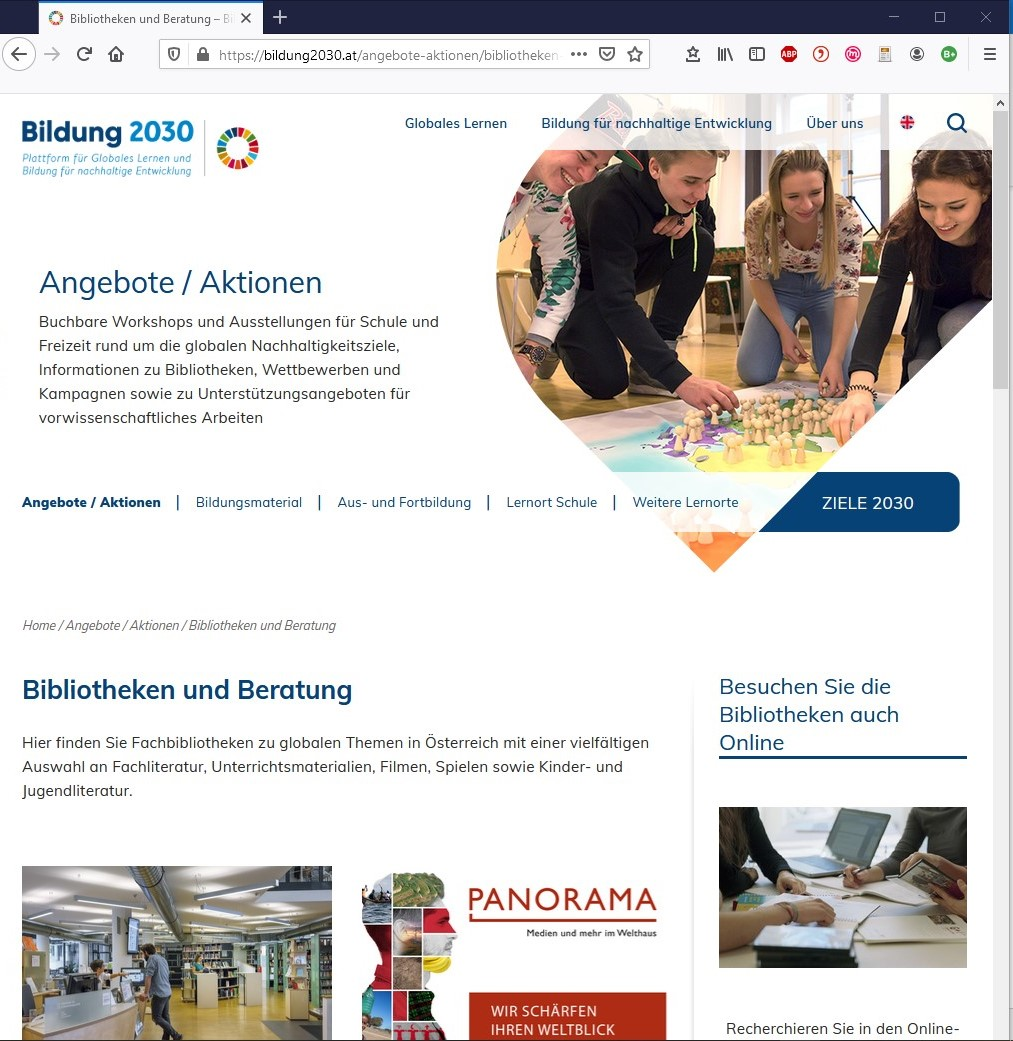
\includegraphics{img/screenshot_1.jpg}
\caption{Die digitale Plattform Bildung 2030 aus Österreich}
\end{figure}

Die Seite besticht durch ihre Funktionalität. Es werden nicht nur Ideen
vermittelt, sondern gleich auch alles Material, Wissen und
Hilfestellungen, welche zur Umsetzung nötig sind. Die
Bibliotheksdienstleistungen wie Zugang zum Katalog oder Beratungen sind
dabei an verschiedenen Unterseiten gut sichtbar eingebettet.
Interessanterweise stellen die Bibliotheken ihre Angebote gar nicht in
den Kontext der Ziele für Nachhaltige Entwicklung. Sie lassen die
Kerndienstleistungen für sich sprechen. Das sind ein Katalogsuchfeld,
persönliche Beratungen und der Bibliotheksbestand an sich. Vergleicht
man diese mit den Best-Practice-Beispielen, findet man diese dort nicht.
Hier sind eher Zusatzelemente wie Ausstellungen oder Aktionstage
vertreten.

Interessant ist auch, dass nur die Bibliotheken, welche das passendste
und umfangreichste Material haben, auf der Plattform bildung2030
vertreten sind. Auf der Seite des Ministeriums sind dann aber
Bibliotheken allgemein genannt. In Österreich haben also diejenigen
Bibliotheken mit der höchsten inhaltlichen Kompetenz die Initiative
ergriffen und ihre Kerndienstleistungen in eine Kooperation eingebracht,
die die Ziele für Nachhaltige Entwicklung allen Interessierten
vermitteln möchte.

\hypertarget{kennen-bibliotheken-die-agenda-2030}{%
\section{Kennen Bibliotheken die Agenda
2030?}\label{kennen-bibliotheken-die-agenda-2030}}

In meinem persönlichen bibliothekarischen Umfeld hatten nur zwei
Personen bereits von den Zielen für Nachhaltige Entwicklung gehört --
eine davon arbeitet regelmässig mit den Verbänden zusammen. Ist es
möglich, dass die Bibliotheken die Ziele für Nachhaltige Entwicklung gar
nicht kennen? Diese Frage liess sich mit der Literaturrecherche nicht
beantworten, dennoch möchte ich an dieser Stelle ein paar Zahlen in den
Raum stellen:

\begin{itemize}
\tightlist
\item
  Auf den Plattformen biblio2030.de und der Library Map of the World
  sind total 34 Beiträge von Bibliotheken aus dem DACH-Raum vermerkt.
\item
  Über die Literaturrecherche sind zusätzlich 35 Best Practice Beispiele
  aus dem DACH-Raum in der Datenbank erfasst.
\item
  Am virtuellen Deutschen Bibliothekstag haben laut der Moderatorin ein
  bisschen mehr als 400 Teilnehmende den Beitrag zu den SDGs gesehen.
  (Breidlind \& Klauser, 2020)
\item
  Im DACH-Raum gibt es total 12.239 Bibliotheken. (IFLA, 2019)
\end{itemize}

Betrachtet man diese Zahlen und nimmt an, dass es keine Überschneidungen
gibt, kann man von rund 470 Bibliotheken ausgehen, die die Ziele für
Nachhaltige Entwicklung kennen. Auf die Gesamtzahl der Bibliotheken
gerechnet, entspricht das rund 4\%.

Diese Zahl deutet darauf hin, dass die meisten Bibliotheken bis jetzt
die Ziele für Nachhaltige Entwicklung noch nicht wahrgenommen haben
beziehungsweise dass deren Einfluss bis jetzt so gering war, dass er nur
bei 4\,\% der Bibliotheken zu einem sichtbaren Einfluss (wie Teilnahme
oder Veröffentlichung von Aktionen) geführt hat. Zumindest wurden
einzelne Bibliotheken erst sehr wenig von den Zielen für Nachhaltige
Entwicklung beeinflusst, soweit das durch Beteiligungen und
Veröffentlichungen messbar ist.

Während in den Verbänden den Zielen für Nachhaltige Entwicklung ein sehr
prominenter Platz zugewiesen wurden, scheinen die einzelnen Bibliotheken
noch nicht viel von ihnen gehört zu haben. Das ist ein starker Kontrast
und man fragt sich, wieso das so stark auseinander geht.

Eine mögliche Ursache liegt vielleicht in der Kommunikation und
Umsetzung der ursprünglichen IFLA-Strategie. Der Schwerpunkt dieser
liegt auf der Interessen- und Öffentlichkeitsarbeit, für welche die
Verantwortung vorwiegend auf Verbandsebene gesehen wird. Bis jetzt haben
die Verbände die einzelnen Bibliotheken im deutschen Sprachraum selten
direkt dazu aufgefordert, die Ziele für Nachhaltige Entwicklung zu
vermitteln. In der direkten Kommunikation zu den Bibliotheken haben die
Verbände die Bibliotheken hauptsächlich dazu aufgerufen, ihre
alltäglichen Bibliotheksdienstleistungen in den Kontext der Ziele für
Nachhaltige Entwicklung zu stellen. Dabei betonten sowohl der dbv als
auch bibliosuisse, dass Bibliotheken bereits mit ihren alltäglichen
Bibliotheksdienstleistungen zur Erfüllung der Ziele für Nachhaltige
Entwicklung beitragen. (Bibliosuisse, 2018; Deutscher Bibliotheksverband
e.\,V., 2020, S. 2)

Eine weitere Ursache könnte in der Komplexität des Themas liegen. Sich
mit den Zielen für Nachhaltige Entwicklung auseinander zu setzen
bedeutet viel Aufwand. Meistens muss man sich erst in das Thema generell
einlesen, bevor man mit den einzelnen Zielen weiterfahren kann. Im
Moment gibt es auch kaum (bibliothekarische) Weiterbildungsangebote zu
den Zielen für Nachhaltige Entwicklung.

\hypertarget{potential-liegt-in-synergien}{%
\section{Potential liegt in
Synergien}\label{potential-liegt-in-synergien}}

Auch wenn die einzelnen Bibliotheken noch nicht so vertraut mit den
Zielen für Nachhaltige Entwicklung sind, gibt es in der
deutschsprachigen Bibliothekswelt viele Gruppen, die sich für diese oder
sehr ähnliche Themen einsetzen. Da wären zum einen die bereits
vorgestellten Bibliotheksverbände und zum anderen das Netzwerk Grüne
Bibliothek und Libraries4Future. Sie alle haben mindestens eine, häufig
sogar mehrere Webseiten, welche Inhalte zu den Themen Nachhaltigkeit
oder zu den Zielen für Nachhaltige Entwicklung bereitstellen. Viele
Inhalte überschneiden sich, jedoch nicht alle. Gleichzeitig wären aber
wohl die meisten Inhalte für alle Interessierten relevant. Während die
unterschiedlichen Trägerinnen inhaltlich leicht verschiedene Ziele haben
und wohl unabhängig voneinander weiter agieren, wäre eine umfassende
Kooperation zum Schwerpunktthema Agenda 2030 sinnvoll.

Dadurch könnten alle Ressourcen sparen und von den Erfahrungen der
anderen profitieren. Wenn eine solche Kooperation eine zentrale
Plattform mit allen Angeboten und Dienstleistungen bereitstellen würde,
könnten auch die Endnutzerinnen und -nutzer davon profitieren. Eine
solche Plattform könnte zum Beispiel die Literaturdatenbank des Netzwerk
Grüne Bibliothek enthalten, die Best-Practice-Sammlungen aller
Kooperationspartnerinnen vereinen und diese mit Hintergrundinformationen
und Materialien anreichern, sodass jede Bibliothek die Aktionen selbst
durchführen kann. Weiterbildungs- und Schulungsmaterialien könnten die
Verbreitung der Ziele für Nachhaltige Entwicklung fördern.

Schlussendlich würden die Gruppen vor allem aber mit gutem Beispiel
vorangehen, und ganz nach den Zielen 4 (Hochwertige Bildung) und 17
(Partnerschaften zur Erreichung der Ziele) handeln.

\hypertarget{literatur}{%
\section{Literatur}\label{literatur}}

BAOBAB -- Globales Lernen. (o.~J.). Bildung2030 -- Plattform für
Globales Lernen und Bildung für nachhaltige Entwicklung. Zugriff am
11.6.2020. Verfügbar unter: \url{https://bildung2030.at/}.

Bibliosuisse. (2018). Bibliosuisse: Kampagne Biblio2030. Verfügbar
unter: \url{https://bibliosuisse.ch/Bibliosuisse/Projekte/Biblio2030}.

Deutscher Bibliotheksverband e.\,V. (o. J.). Plattform biblio2030.de.
Zugriff am 30.5.2020. Verfügbar unter: \url{https://www.biblio2030.de/}.

Deutscher Bibliotheksverband e.\,V. (Hrsg.). (2020, April). Bibliotheken
und Nachhaltigkeit: Praktische Beispiele zum Beitrag von Bibliotheken zu
den Nachhaltigkeitszielen. Verfügbar unter:
\url{https://www.bibliotheksverband.de/fileadmin/user_upload/DBV/publikationen/200429_dbv-Flyer_Web-Ansicht_150dpi.pdf}.

IFLA. (2015). Bibliotheken und die Umsetzung der UN 2030 Agenda.
Verfügbar unter:
\url{https://www.ifla.org/files/assets/hq/topics/libraries-development/documents/libraries-un-2030-agenda-toolkit-de.pdf}.

IFLA. (2019). \emph{IFLA Map of the World - SDG Stories Map}. Verfügbar
unter: \url{https://librarymap.ifla.org/stories}.

IFLA. (2020). IFLA: Libraries, Development and the United Nations 2030
Agenda. Zugriff am 31.5.2020. Verfügbar unter:
\url{https://www.ifla.org/libraries-development}.

United Nations. (o. J.). Sustainable Development Knowledge Platform.
Verfügbar unter: \url{https://sustainabledevelopment.un.org/}.

%autor
\begin{center}\rule{0.5\linewidth}{0.5pt}\end{center}

\textbf{Franziska Corradini} ist gelehrte Fachfrau Information und
Dokumentation. Im Herbst hat sie das Studium Informationswissenschaft an
der Fachhochschule Graubünden abgeschlossen. Sie arbeitet in der
Mediothek IWM der PHBern in den Bereichen Kundendienst, Schulungen und
Ausstellungen.

\end{document}
